To verify that the proposed architecture works, we implement a simple Euclidean distance calculation on trajectories. For this the data needs to be pre-processed and the events should be matched with location from cell map data set.

\subsection{Experimental setup}
The experiments were executed in a Mac Book Pro with the following characteristics: 2,6 GHz Intel Core i5, 8 GB 1600 MHz DDR3 memory and 256 GB of storage.

\subsection{Data sets}
The following data sources are used:
\begin{itemize}
\item Cell map Data: OpenCelliD public data set representing cell tower locations and meta data.
\item CDR data: Sequences of network connections together with actual GPS location (recording every second the information about neighbouring cell towers including the connected one)
\end{itemize}

\subsubsection{Cell map data set}
The full data set of OpenCelliD was downloaded as of 2018-05-26. The downloaded .csv file is 3.38 GB on disk. The following attributes of OpenCelliD data set are used for the analysis \cite{opencellid}:
\begin{itemize}
\item radio: \textit{string} - Network type. One of the strings GSM, UMTS, LTE or CDMA.
\item mcc:  \textit{integer}  -  Mobile Country Code, for example 262 for Germany.
\item net: \textit{integer} - For GSM, UMTS and LTE networks, this is the Mobile Network Code (MNC). For CDMA networks, this is the System Identification number (SID).
\item cell: \textit{integer} - Cell ID (CID) for GSM and LTE networks. UTRAN Cell ID / LCID for UMTS networks, which is the concatenation of 2 or 4 bytes of Radio Network Controller (RNC) code and 4 bytes of Cell ID. Base station identifier number (BID) for CDMA networks.
\item lat: \textit{double} - Latitude in degrees between -90.0 and 90.0.
\item lon: \textit{double} - Longitude in degrees between -180.0 and 180.0.
\item samples: \textit{integer} - Total number of measurements assigned to the cell tower.
\item changeable:  \textit{integer} - Defines if coordinates of the cell tower are exact or approximate. \footnote{changeable=1: the GPS position of the cell tower has been calculated from all available measurements. changeable=0: the GPS position of the cell tower is precise - no measurements have been used to calculate it.}
\item created: \textit{integer} - The first time when the cell tower was seen and added to the OpenCelliD database. \footnote{A date in time stamp format: number of seconds since the UTC Unix Epoch of 1970-01-01T00:00:00Z (For example 1409522613 is the time stamp for 2014-08-31T22:03:33Z).}
\item updated: \textit{integer} - The last time when the cell tower was seen and updated.
\end{itemize}

We expect less cell towers in the outskirts of the city and more towards the center. Figure \ref{fig:opencellid}\footnote{Only the latest observations are shown.} shows that the density of cell towers within Telfonica network from OpenCelliD is quite dense even in the outer regions of Berlin. Thus the data from OpenCelliD might be corrupted or of poor quality.

\begin{figure}[h]
    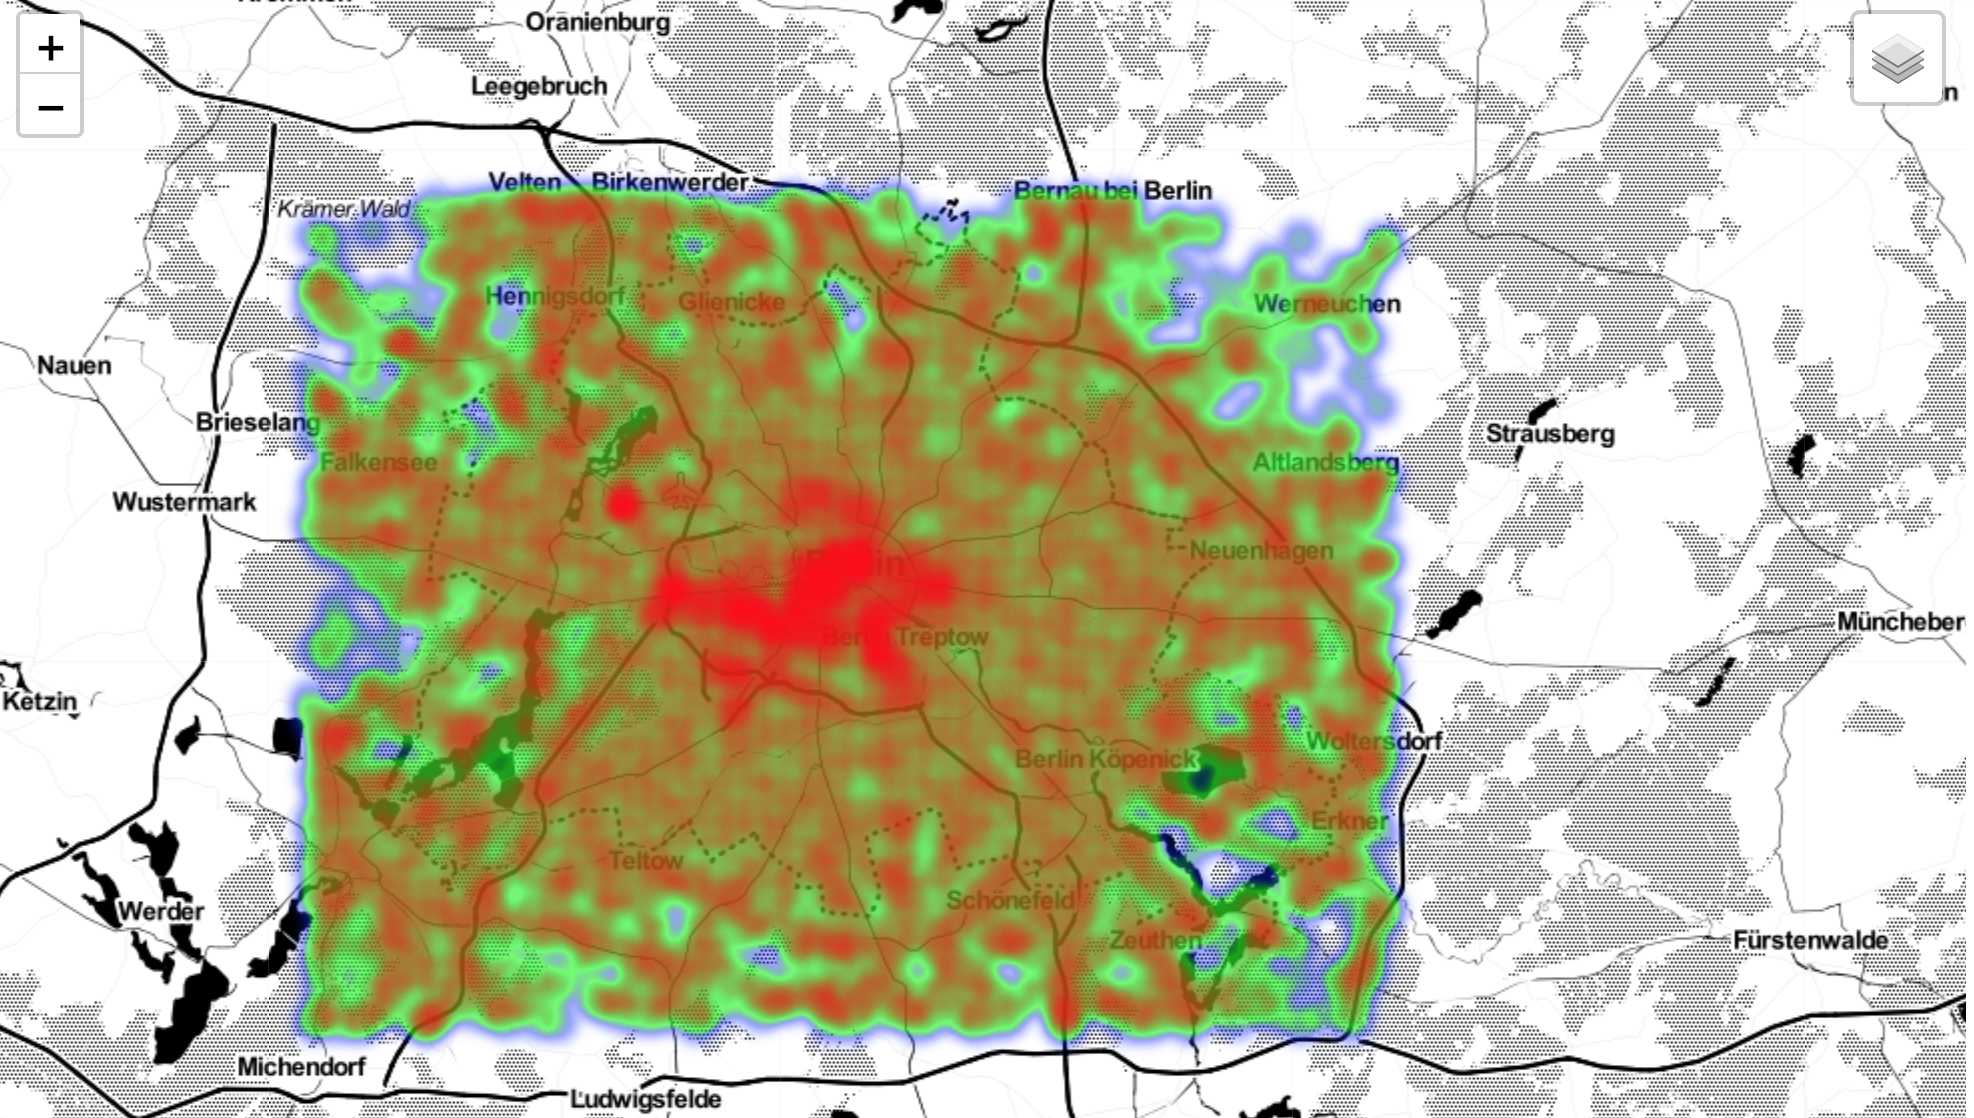
\includegraphics[width=0.45\textwidth]{images/opencellid.png}
    \caption{Heat map of Telefonica cell towers in Berlin (Source: OpenCelliD) }
    \label{fig:opencellid}
\end{figure}

\subsubsection{CDR data}
The CDR data set was generated for several days between 2018-05-08 and 2018-05-17 in Berlin region with a custom application using Samsung S8 test phone (Android operating system). The generated .csv file is 2.21 gigabytes. The CDR data includes features such as:
\begin{itemize}
\item system\_time: \textit{integer} - Date and time when event was generated in timestamp format, i.e. the number of seconds since Jan 01 1970. (UTC)
\item unix\_dt: \textit{datetime} - Date and time when event was generated.
\item net: \textit{string} - Type of the network (e.g. GSM, LTE or UMTS).
\item lac: \textit{integer} - Location Area Code of the cell.
\item cisac: \textit{integer} - Cell id.
\item latitude: \textit{double} - Latitude of actual GPS location of the phone.
\item longitude: \textit{double} - Longitude of actual GPS location of the phone.
\end{itemize}

There are cell towers that were assigned to the collected events more frequently than others. These are likely to be around the home or workplace of the user generating the data.

On average there was a CDR record logged in about every second during the data collection. However that would be less frequent with real life usage, depending on individual mobile usage preferences. 

By collecting observation in every second, we discretize time and make sure that the trajectories we compare using Euclidean distance have the same number of data points.

\subsection{Data pre-processing}
The cell map data cannot be processed with Pandas due to its size, therefore pySpark is used for the cleaning process with the following steps: 
\begin{enumerate}
    \item Import csv to pySpark DataFrame
    \item Drop irrelevant columns
    \item Keep only the records of cells in the Telefonica network in Berlin
    \item Write cleaned data to parquet files
\end{enumerate}

The data-flow throughout the implementation steps can be seen on Figure \ref{fig:data-flow}.
\begin{figure}[h]
    \centering
    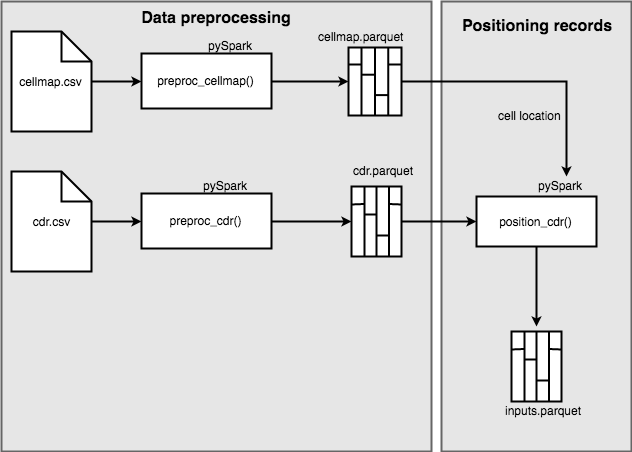
\includegraphics[width=0.45\textwidth]{images/data-flow.png}
    \caption{Data flow diagram}
    \label{fig:data-flow}
\end{figure}

The CDR data-set generated by the test phone in the given time period is stored in a single .csv file. The size of the file is around fifty megabytes, given only one device was used to record logs. However the size of real-world mobile network events generated daily can go up to hundreds of gigabytes per day. The following steps are executed during the pre-processing: 
\begin{enumerate}
   \item Import .csv files to pySpark DataFrame
    \item Clean data:
    \begin{itemize}
        \item Fetch data from JSON column to data frame columns
        \item Create cell(lac, cisac) column
    \end{itemize}
    \item Write data to Parquet files
\end{enumerate}

The DataFrames are re-partitioned before writing them to Parquet files to avoid having a large number of tiny files for a relatively small data. 

\subsection{Positioning mobile network events}
Having preprocessed the raw data, the next step is to assign a location to each of the events in the CDR data-set from the cell map data-set based on the respective cell tower id. 
These steps are executed for positioning the CDR data:
\begin{itemize}
    \item Load CDR data from parquet files to pySpark DataFrame
    \item Load cell map data from Parquet to pySpark DataFrame
    \item Prepare imported DataFrames
    \item Join CDR and cell map data-sets on cell id
    \item Calculate Haversine distances
    \item Persist joined DataFrame to parquet files
\end{itemize}

\subsection{Trajectory distance calculation}
As the users tend to move while using their phones, the generated CDR observations have semantics of trajectories. CDR data points can be grouped as trajectories so that the characteristics of trajectories and the result of previous research already conducted in this field can be utilized for achieving more accurate positioning.

To evaluate cellular network event based customer localization we calculate the Euclidean distance and the edit distance along with several statistics of the pairwise distances between ground truth GPS trajectories and mobile network event trajectories. The Haversine distance is used to define the spatial distance between points. In the mobile network event trajectory, the location information is obtained from cell map data set.

Similarly to the formulation in \cite{encyclopedia} and \cite{distance-def} we define distance measure on trajectories, such as:
\begin{definition}
Let $\mathcal{M}$ be a set of trajectories. A function $D :\mathcal{M} \times \mathcal{M} \rightarrow \mathcal{R}$ \nomenclature{$D$}{Distance measure defined on a set of trajectories.} is called a dissimilarity (distance) on $\mathcal{M}$ if for all $T_{1}, T_{2} \in \mathcal{M}$: 
\begin{itemize}
    \item $D(T_{1},T_{2}) \geqslant 0$
    \item $D(T_{1},T_{2}) = d(T_{2},T_{2})$
    \item $D(T_{1},T_{1}) = 0$
\end{itemize}
If all of these conditions are satisfied and $D(T_{1}, T_{2}) = 0 \Rightarrow  T_{1} = T_{2} $ is considered to be a symmetric. If
the triangle inequality is also satisfied, $D$ is a metric.
\end{definition}

The \textit{Euclidean distance} (or inverse similarity) measure between two trajectories is used in this analysis:
\[D(T,\Tilde{T}) = \sqrt{\sum_{i=1}^{n} (d(P_{i},\Tilde{P_{i}}))^{2}}\]

where $d((P_{i},\Tilde{P_{i}})$ refers to the spatial distance between two points given with the Haversine formula.

The Euclidean distance algorithm presented in Algorithm \ref{algo:euclidean} is implemented with Pandas UDFs invoked on PySpark data frames. Pandas UDFs convert the columns of Spark data frames into Pandas Series and they also return Pandas Series, which eliminates row by row iteration in contrast with standard UDFs in PySpark.

\begin{algorithm}
\begin{algorithmic}
\caption{Euclidean distance function on trajectories} \label{algo:euclidean}
\Function{euclideanDist}{Traj tReal, Traj tApprox}
\State dEuclidean = 0
\State nPoints = len(tReal) 
\For{i \textbf{in} 0 to nPoints}
    \State dEuclidean = dEuclidean + power(haversine(     
    \State tReal[i], tApprox[i]) , 2)
\EndFor
\Return sqrt(dEuclidean)
\EndFunction
\end{algorithmic}
\end{algorithm}


\subsection{Experiments}
We define two types of performance tests. For different Spark standalone clusters we compare the runtime of
\begin{itemize}
    \item the standard Spark UDFs and the newly added Pandas UDFs (PUDF) implementation of Euclidean distance on two trajectories for several days,
    \item common PySpark data frame operators - such as filtering, joining, counting and sorting - using different data sources, namely comma separated value files and Parquet files. 
\end{itemize}

The specifications of the clusters are shown in Table \ref{tab:spec}.
\begin{table}[h]
    \centering
    \resizebox{0.45\textwidth}{!}{%
    \begin{tabular}{|l|c|c|c|}
    	\hline
         & \textbf{Cluster A} & \textbf{Cluster B} & \textbf{Cluster C}\\
        \hline 
        \# of workers & 1 & 2 & 1 \\
        \hline
        Worker cores  & 1 & 1 & 2 \\
        \hline
        Worker memory & 1GB & 2GB & 2GB \\
        \hline
        Driver memory & 1GB & 1GB & 1GB \\
        \hline
        Executor memory & 512MB & 1GB & 1GB \\
        \hline
    \end{tabular}}
    \caption{Specifications of test clusters}
    \label{tab:spec}
\end{table}

Worker memory is the total amount of memory and worker core is the number of cores Spark applications are allowed to use on the machine. Driver memory refers to the amount of memory to use for the driver process, which is where the SparkContext is initialized. Spark executor memory is the amount of memory to use per executor process. \cite{spark:rdds}

First we compare the performance of Pandas and Spark data frames over the several days in terms of the runtime of a simple Euclidean distance calculation between two trajectories.

Then we test the performance of data frame operations with .csv and Parquet storage formats. Since Spark applications are lazily evaluated, a count() operation was called on the resulting DataFrames to reliably reflect the execution time.

\subsection{Results}
The results of the comparison of the standard Spark UDFs and the Pandas UDFs (PUDF) implementation of Euclidean distance on two trajectories for several days is shown in Table \ref{tab:spark-pd}. The larger the number of rows is, the more significant the improvement is. For all dates, the runtime of the Pandas UDF implementation with Cluster A is approximately eight times less than the runtime of the standard UDF. This is due to the fact that Pandas UDFs are not iterating over the rows, but use vectorized operations instead. Thus for large row count Pandas UDFs are more efficient than the standard UDFs. 

Cluster B increases the runtime of both UDF and Pandas UDF implementations, as it adds more networking overhead with the additional worker, which is not balanced by the parallelism. Cluster B and C have similar performance, which means that for UDFs, the higher number of cores does not necessarily result in better performance.

\begin{table}[h]
    \centering
    \resizebox{0.48\textwidth}{!}{%
    \begin{tabular}{|l|c|c|c|c|c|c|c|}
        \hline
         &  & \multicolumn{2}{c|}{\textbf{Cluster A}} & \multicolumn{2}{c|}{\textbf{Cluster B}} & \multicolumn{2}{c|}{\textbf{Cluster C}}\\
    	\hline
        \textbf{Date} & \textbf{Count} & \textit{UDF} & \textit{PUDF} &\textit{UDF} & \textit{PUDF} &\textit{UDF} & \textit{PUDF} \\
        \hline
        2018-05-08 & 88381 & 5.93  & 5.44 & 10.42 & 6.07 & 6.21 & 6.23 \\
        \hline
        2018-05-09 & 724101 & 15.68 & 6.45 & 14.81 & 6.70 & 12.56 & 7.55 \\
        \hline
        2018-05-10 & 388715 & 8.76 & 5.81 & 10.29 & 8.38 & 8.81 & 7.78 \\
        \hline
        2018-05-11 & 689603 & 13.25 & 5.73 & 12.49 & 6.92 & 12.04 & 7.78 \\
        \hline
        2018-05-13 & 1039702 & 18.50 & 6.24 & 15.68 & 7.28 & 15.44 & 7.69 \\
        \hline
        2018-05-14 & 135989 & 5.91 & 5.30 & 7.67 & 6.98 & 7.51 & 6.47 \\
        \hline
        2018-05-15 & 416399 & 10.38 & 5.47 & 9.76 & 6.69 & 9.36 & 6.86 \\
        \hline
        2018-05-16 & 43342 & 5.60 & 5.86 & 6.66 & 6.06 & 5.52 & 6.38 \\
        \hline
        2018-05-17 & 32799 & 5.03 & 5.74 & 6.48 & 6.72 & 5.24 & 6.56 \\
        \hline
        \textbf{All dates} & \textbf{3641574} & \textbf{59.45} & \textbf{7.15} & \textbf{35.01} & \textbf{8.38} & \textbf{40.05} & \textbf{8.02} \\
        \hline
    \end{tabular}}
    \caption{Run-times of data processing tasks with different test clusters in seconds}
    \label{tab:spark-pd}
\end{table}

The execution time of the common data frame operators in Spark with two different storage formats can be seen in Table \ref{tab:res}.

It is obvious that .csv is not optimal storage format for big data processing. However in many cases data is available in .csv only, so it needs to be converted to Parquet for better efficiency. 

\begin{table}[h]
    \centering
    \resizebox{0.48\textwidth}{!}{%
    \begin{tabular}{|l||c|c|c|c|c|c|}
    	\hline
        \textbf{Task name} & \multicolumn{2}{c|}{\textbf{Cluster A}} & \multicolumn{2}{c|}{\textbf{Cluster B}} & \multicolumn{2}{c|}{\textbf{Cluster C}}\\
        \hline
        \textit{Data source} & \textit{parquet} & \textit{.csv} & \textit{parquet} & \textit{.csv} & \textit{parquet} & \textit{.csv}\\
        \hline 
        \hline
        read\_data() & 29.17 & 247.70 & 27.79 & 142.92 & 23.31 & 167.39 \\
        \hline
        min\_of\_col() & 14.58 & 76.07 & 10.01 & 74.20 & 11.33 & 55.15 \\
        \hline
        sort\_by\_col() & 71.75 & 198.81 & 53.35  & 161.16 & 47.10 & 136.64 \\
        \hline
        filter\_by\_col() & 3.94 & 91.14 & 3.59 & 69.85 & 3.47 & 55.01 \\
        \hline
        join\_dfs() & 44.69 & 167.56 & 30.38 & 123.29 & 27.57 & 107.08\\
        \hline
        collect\_rows() & 3.05 & -\footnotemark & 2.86 & -\footnotemark & 2.31 & -\footnotemark \\
        \hline
        \textbf{Total} & \textbf{167.18} & \textbf{781.28} & \textbf{127.97} & \textbf{571.42} & \textbf{115.09} & \textbf{521.27} \\
        \hline
    \end{tabular}}
    \caption{Run-times of data processing tasks with different test clusters in seconds}
    \label{tab:res}
\end{table}
\footnotetext{Running collect\_rows() method,'java.lang.OutOfMemoryError: Java heap space' occurs.}
\footnotetext{Running collect\_rows() method,'ConnectionRefusedError' occurs, indicating that an error occurred while trying to connect to the Java server.}

Cluster C has the shortest runtime, which means that for the data frame operations in this test, adding more cores instead of more workers results in the best performance for both storage formats. 

With this architecture design, it is reasonably easy to deploy the application on Amazon Web Services (AWS) or similar cloud service provider allowing scalability to process terabytes of data.

